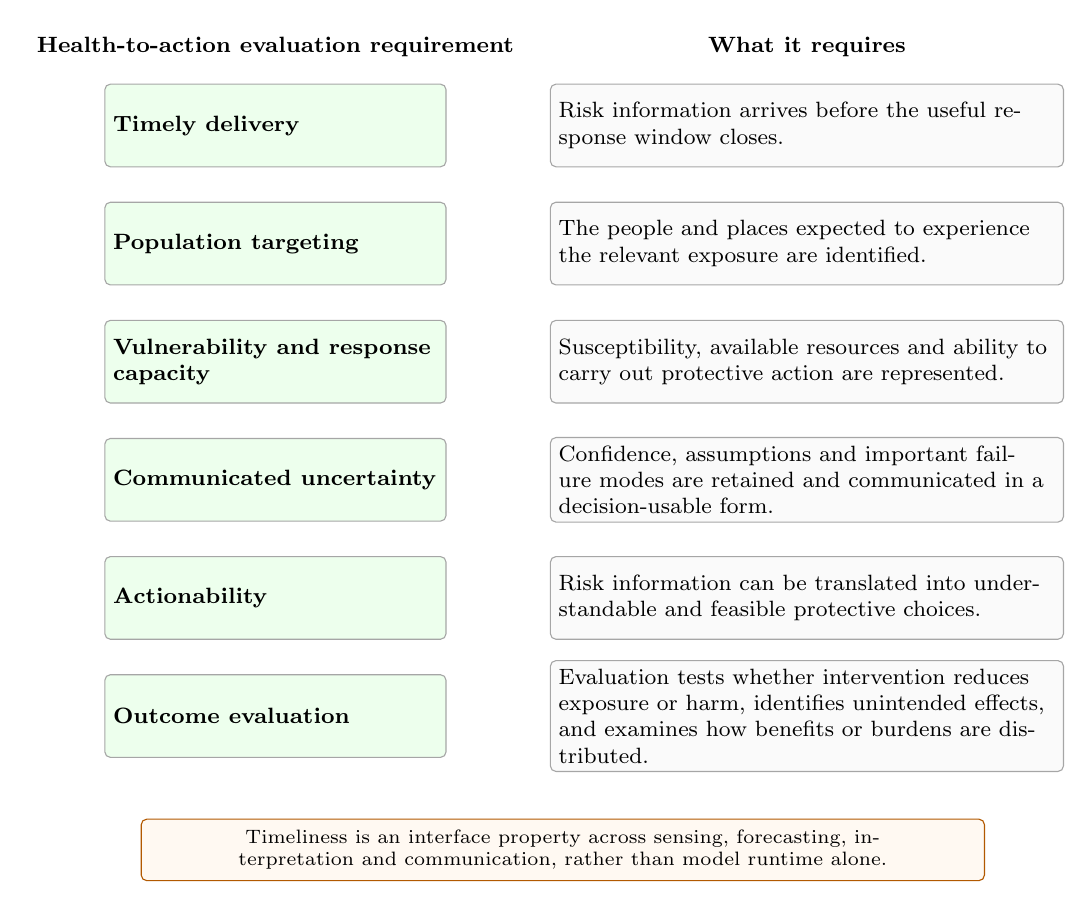
\begin{tikzpicture}[
row/.style={draw=black!35,rounded corners=2pt,minimum height=10.5mm,inner sep=3pt,font=\footnotesize,text=black},
req/.style={row,fill=green!7,align=left,text width=0.34\linewidth,font=\bfseries\footnotesize},
meaning/.style={row,fill=black!2,align=left,text width=0.52\linewidth},
head/.style={font=\bfseries\footnotesize,text=black}
]
\node[head] at (2.35,0.45) {Health-to-action evaluation requirement};
\node[head] at (9.10,0.45) {What it requires};
\node[req] (r1) at (2.35,-0.55) {Timely delivery};
\node[meaning] (m1) at (9.10,-0.55) {Risk information arrives before the useful response window closes.};
\node[req] (r2) at (2.35,-2.05) {Population targeting};
\node[meaning] (m2) at (9.10,-2.05) {The people and places expected to experience the relevant exposure are identified.};
\node[req] (r3) at (2.35,-3.55) {Vulnerability and response\\capacity};
\node[meaning] (m3) at (9.10,-3.55) {Susceptibility, available resources and ability to carry out protective action are represented.};
\node[req] (r4) at (2.35,-5.05) {Communicated uncertainty};
\node[meaning] (m4) at (9.10,-5.05) {Confidence, assumptions and important failure modes are retained and communicated in a decision-usable form.};
\node[req] (r5) at (2.35,-6.55) {Actionability};
\node[meaning] (m5) at (9.10,-6.55) {Risk information can be translated into understandable and feasible protective choices.};
\node[req] (r6) at (2.35,-8.05) {Outcome evaluation};
\node[meaning] (m6) at (9.10,-8.05) {Evaluation tests whether intervention reduces exposure or harm, identifies unintended effects, and examines how benefits or burdens are distributed.};
\node[draw=orange!70!black,fill=orange!5,rounded corners=2pt,align=center,text width=0.86\linewidth,inner sep=4pt,font=\scriptsize,text=black] at (6.0,-9.75)
{Timeliness is an interface property across sensing, forecasting, interpretation and communication, rather than model runtime alone.};
\end{tikzpicture}
